\chapter{셸과 스크립팅}

\section{기본 개요}
\subsection*{터미널}
\begin{flushleft}
    \textbf{터미널}은 텍스트로 된 사용자 인터페이스를 제공하는 프로그램이다.
    터미널은 키보드에서 문자를 읽어 화면에 표시하는 기능을 지원한다.
    초창기(Unix 시절)에는 하나의 메인프레임에 접속하기 위한 모니터와 키보드가 통합된 장치였으나
    현재는 앱일 뿐이다.
    그런 흔적이 tty(teletype)로 /dev 하위에 남아있다.
\end{flushleft}

\subsection*{셸}
\begin{flushleft}
    \textbf{셸}(shell)은 스트림을 통해 입력, 출력을 처리하고, 변수를 지원하며,
    사용 가능한 내장(built-in) 명령이 몇가지 있으며, 명령 실행 상태 및 상태를 처리하고,
    일반적으로 대화식 사용과 스크립트 사용을 모두 지원한다.
\end{flushleft}

\begin{flushleft}
    공식적으로 셸은 \textbf{sh}로 정의하며, POSIX 셸이라는 용어를 접하게 되는데,
    이는 스크립트와 이식성 맥락에서 중요하다.
    초기에는 창안자의 이름을 딴 본 셸(Bourne Shell, sh)이 많이 쓰였지만,
    최근에는 bash 셸(Bourne again shell)을 주로 사용한다.
\end{flushleft}

\begin{flushleft}
    어떤 셸이 사용되고 있는지 궁금하면 file -h /bin/sh 명령을 사용해 확인해보고,
    만약 이 명령이 실패하면 echo \$0 또는 echo \$SHELL을 시도해보자.
\end{flushleft}

\begin{flushleft}
    이어서 스트립과 변수라는 두 가지 기본 기능에서 출발해
    셸의 기본 기능을 알아보자.
\end{flushleft}

\subsubsection*{스트림}
\begin{flushleft}
    셸은 입력과 출력을 위한 세 가지 기본 파일 디스크립터(File Descriptor, FD)를 모든 프로세스에 제공한다.
\end{flushleft}

\begin{itemize}
    \item stdin (FD 0)
    \item stdout (FD 1)
    \item stderr (FD 2)
\end{itemize}

\begin{flushleft}
    이 FD들은 그림 \ref{fig:stream}에 나와 있는 것처럼
    기본적으로 화면과 키보드에 각각 연결되어 있다.
    즉 특별하게 지정하지 않는 한,
    셸에 입력하는 명령은 키보드에서 입력(stdin)을 가져오고 출력(stdout)을 화면에 전달한다.
    다음 셸의 상호작용에서 위의 기본 동작을 확인할 수 있다.
\end{flushleft}

\begin{figure}[h]
    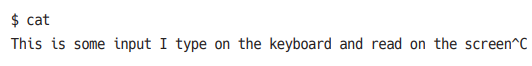
\includegraphics[width=15cm]{resource/3-stream-example}
    \label{fig:stream-example}
\end{figure}

\begin{flushleft}
    cat을 사용한 방금의 예에서 기본값이 동작하는 것을 확인할 수 있다.
    그리고 Ctrl+c를 사용해 명령을 종료했다.
\end{flushleft}

\begin{figure}[h]
    \centering
    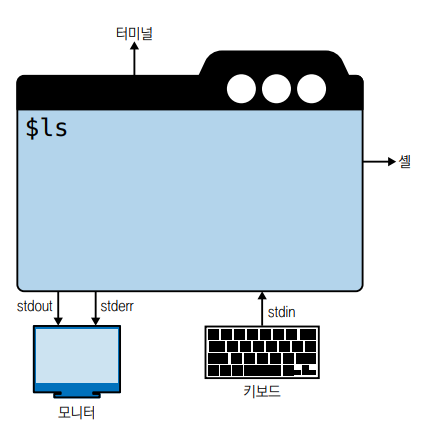
\includegraphics[width=8cm]{resource/3-2}
    \caption{셸 I/O의 기본 스트림}
    \label{fig:stream}
\end{figure}

\begin{flushleft}
    셸이 제공하는 기본값을 사용하지 않으려면 스트림을 재지정(redirect)할 수 있다.
\end{flushleft}

\begin{flushleft}
    \$FD$>$와 $<$\$FD를 사용해 프로세스의 출력 스트림을 재지정할 수 있다.
    여기서 \$FD는 파일 디스크립터다.
    예를 들어 2$>$는 stderr 스트림을 재지정한다는 의미다.
    1$>$는 $>$는 stdout이 기본값이므로 동일한 뜻이다.
    stdout과 stderr를 모두 재지정하러면 \&$>$를 사용하고
    스트림을 제거하려면 /dev/null을 사용하면 된다.
    구체적인 예를 들어 이 사항이 어떻게 동작하는지 살펴보자.
    아래는 curl을 통해 HTML 콘텐츠를 다운로드 하는 예제이다.
\end{flushleft}

\begin{figure}[h]
    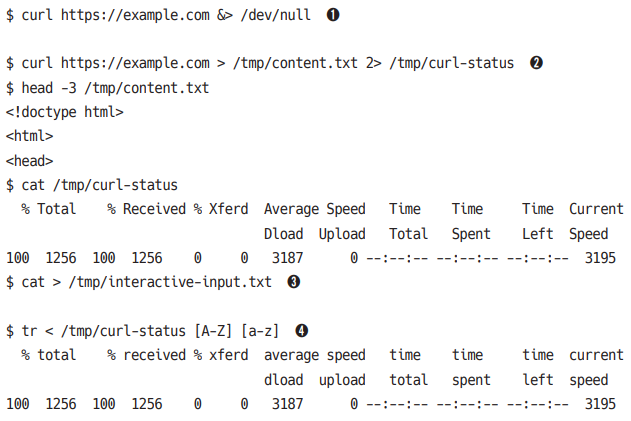
\includegraphics[width=15cm]{resource/3-curl-stream}
\end{figure}

\begin{enumerate}
    \item stdout과 stderr을 모두 /dev/null로 재지정해 모든 출력값을 버린다.
    \item 출력값과 상태값을 다른 파일로 재지정한다.
    \item 대화식으로 값을 입력하고 파일에 저장한다.
        Ctrl+d를 사용해 캡처를 중지하고 콘텐츠를 저장한다.
    \item stdin에서 값을 읽는 tr 명령을 사용해 모든 단어를 소문자로 만든다.
\end{enumerate}

\begin{flushleft}
    셸은 일반적으로 다음과 같은 여러 특수 문자를 이해한다.
\end{flushleft}

\begin{itemize}
    \item \textbf{앰퍼샌드}(\&)\newline
        명령 마지막에 배피되며 백그라운드에서 명령을 실행한다.
    \item \textbf{백슬래시}(\textbackslash)\newline
        긴 명령의 가독성을 높이기 위해 다음 행에서 명령을 계속할 때 사용한다.
    \item \textbf{파이프}(\textbar)\newline
        한 프로세스의 stdout 값을 다음 프로세스의 stdin과 연결해 데이터를
        파일에 임시로 저장하지 않고 바로 전달할 수 있다.
\end{itemize}

\begin{flushleft}
    파이프는 매우 많은 사항을 내포하고 있다.
    파이프와 관련된 사항은 다음 \href{https://web.cse.ohio-state.edu/~mamrak.1/CIS762/pipes_lab_notes.html}{유닉스 파이프}를 참고하고
    유닉스와 마이크로서비스 사이 유사성을 다룬 \href{https://opensource.com/article/18/11/revisiting-unix-philosophy-2018}{2018년 유닉스 철학 재조명} 기사도 참고하면 좋다.
\end{flushleft}


\subsubsection*{변수}
\begin{flushleft}
    값을 하드코딩하고 싶지 않거나 불가능할 때는 언제든 변수를 사용해 값을 저장하고 변경할 수 있다.
    사용 예는 다음과 같다.
    \begin{itemize}
        \item 리눅스가 노출하는 구성 항목을 처리하려는 경우
            (ex - 셸이 \$PATH 변수에 저장된 실행 파일을 찾는 위치).
            이는 변수를 읽기/쓰기할 수 있는 일종의 인터페이스다.
        \item 스크립트에서 사용자에게 값을 대화 형식으로 질문하려는 경우 
        \item 긴 값을 한 번 정의해 입력을 줄이려는 경우(ex - HTTP API의 URL).
            이 사용 사례는 변수를 선언한 후 값을 변경하지 않기 때문에
            대략적으로 프로그램 언어의 const 값에 해당한다.
    \end{itemize}
\end{flushleft}

\begin{flushleft}
    변수는 다음과 같이 두 가지 종류로 나뉜다.
    \begin{itemize}
        \item \textbf{환경변수}\newline
            셸 전체의 설정.
            env 명령어로 목록을 나열한다.
        \item \textbf{셸 변수}\newline
            현재 실행 상황에서 유효하다.
            bash에서 set 명령어로 목록을 나열할 수 있다.
            하위 프로세스는 셸 변수를 상속하지 않는다.
    \end{itemize}
\end{flushleft}

\begin{flushleft}
    배시에서 export 명령어를 사용해 환경 변수를 만들 수 있다.
    변수의 값에 접근하고 싶을 때는 앞에 \$를 붙이고,
    변수를 제거하고 싶을 때는 unset을 이용한다.
\end{flushleft}

\begin{flushleft}
    실제로 어떻게 보이는지 살펴보자.
\end{flushleft}

\begin{figure}[H]
    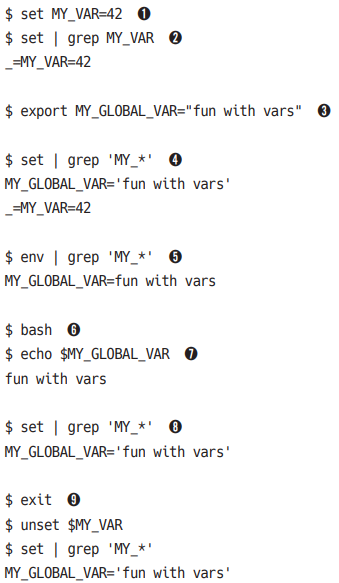
\includegraphics[width=8cm]{resource/3-variable}
    \label{fig:variable}
    \begin{enumerate}
        \item MY\_VAR라는 셸 변수를 생성하고 값을 42로 지정한다.
        \item 셸 변수를 나열하고 MY\_VAR를 필터링 한다.
            환경변수로 내보내지 않았음을 나타내는 \_=에 유의하자.
        \item MY\_GLOBAL\_VAR라는 새 환경변수를 만든다.
        \item 셸 변수를 나열하고 MY\_로 시작하는 모든 변수를 필터링해본다.
            예상대로 이전 단계에서 만든 두 변수가 모두 표시된다.
        \item 환경변수를 나열한다. 예상대로 MY\_GLOBAL\_VAR이 표시된다.
        \item 새 셸 세션,
            즉 MY\_VAR을 상속하지 않는 현재 셸 세션의 자식 프로세스를 만든다.
        \item 환경변수 MY\_GLOBAL\_VAR에 접근한다.
        \item 현재 자식 프로세스에 있기 때문에 셸 변수를 나열하면
            MY\_GLOBAL\_VAR만 나온다.
        \item 자식 프로세스를 종료한 후 MY\_VAR 셸 변수를 제거하고 셸 변수를 나열한다.
            예상대로 MY\_VAR이 사라졌다.
    \end{enumerate}
\end{figure}

\begin{table}[H]
    \everyrow{\hline}
    \begin{tabu}{|X[3]|X[2]|X[12]|}
        변수         &    유형      & 의미    \\
        EDITOR      &   POSIX     & 파일 편집 시 기본적으로 사용되는 프로그램의 경로 \\
        HOME        &   배시 셸    & 현재 사용자의 홈 디렉터리 경로 \\
        HOSTNAME    &   POSIX     & 현재 호스트의 이름 \\
        IFS         &   POSIX     & 필드를 구분할 문자 목록, 셸이 단어를 확장해서 분할할 떄 사용함 \\
        PATH        &   POSIX     & 셸이 실행 가능한 프로그램을 찾는 디렉터리 목록을 포함 \\
        PS1         &   환경       & 사용 중인 주 프롬프트 문자열 \\
        PWD         &   환경       & 작업 디렉터리의 전체 경로 \\
        OLDPWD      &   배시 셸    & 마지막 cd 명령을 실행하기 직전의 디렉터리 경로 \\
        RANDOM      &   배시 셸    & 0에서 32767 사이의 임의의 정수 \\
        SHELL       &   환경       & 현재 사용되는 셸 \\
        TERM        &   환경       & 사용하는 터미널 에뮬레이터 \\
        UID         &   환경       & 현재 사용자의 고유 ID(정수) \\
        USER        &   환경       & 현재 사용자 이름 \\
        \_          &   배시 셸    & foreground에서 실행된 이전 명령의 마지막 인수 \\
        ?          &   배시 셸    & 종료 상태 \\
        \$          &   배시 셸    & 현재 프로세스의 ID(정수) \\
        0           &   배시 셸    & 현재 프로세스의 이름 \\
    \end{tabu}
    \caption{일반적인 셸 변수와 환경변수}
    \label{tab:variable}
\end{table}

\begin{flushleft}
    표 \ref{tab:variable}에 일반적인 셸과 환경 변수를 정리했다.
    이 환경변수들은 거의 모든 곳에서 찾을 수 있으며,
    잘 이해하고 사용하는 것이 중요하다.
    모든 변수에 대해 echo \$XXX 명령을 사용하면 해당 값을 볼 수 있는데
    여기서 XXX는 변수 이름이다.
\end{flushleft}

\subsubsection*{종료상태}
\begin{flushleft}
    셸은 \textbf{종료 상태}(exit status)라고 하는 것을 사용해 명령 실행 완료를 명령 호출자에게 알린다.
    일반적으로 리눅스 명령은 종료될 때 상태를 반환한다.
    이는 정상적인 종료(원활한 경로 또는 happy path라고 부름)일 수도 비정상 종료일 수도 있다.
    종료 상태값 0은 명령이 오류 없이 성공적으로 실행됬음을 의미하는 반면
    1에서 255 사이의 값은 실패를 나타낸다.
    종료 상태를 확인하려면 echo \$?를 사용한다.
\end{flushleft}

\begin{flushleft}
    일부 셸에서는 마지막 상태값만 사용할 수 있으므로
    파이프 사용 시 종료 상태 처리에 주의해야 한다.
    \$PIPESTATUS를 사용하면 이런 제약사항을 해결할 수 있다.
\end{flushleft}

\subsubsection*{내장 명령어}
\begin{flushleft}
    셸에는 여러 내장 명령어(built-in command)가 있다.
    몇 가지 유용한 예로는 yes, echo, cat, read가 있다.
    help 명령을 사용하면 내장 명령어 목록을 나열할 수 있다.
    그러나 그 외 모든 것은 보통 /usr/bin(사용자 명령의 경우)나 /usr/sbin(관리 명령의 경우)에 있는
    셸 외부 프로그램이라는 점을 기억하자.
    그러면 실행 파일을 어디에서 찾을지 어떻게 알 수 있을까?
    다음과 같은 방법이 있다.
\end{flushleft}

\begin{figure}[H]
    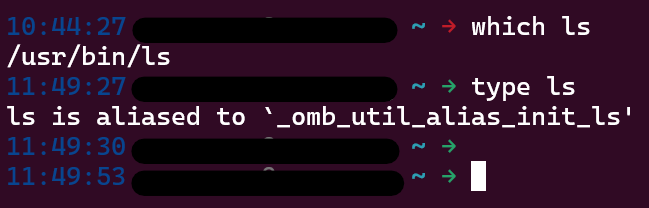
\includegraphics[width=15cm]{resource/3-built-in}
    \caption{실행 파일 위치 확인 예시}
    \label{fig:build-in}
\end{figure}


\subsubsection*{작업 제어}
\begin{flushleft}
    \textbf{작업 제어}는 대부분의 셸이 지원하는 기능이다.
    기본적으로 명령을 입력하면 그 명령은 일반적으로 화면과 키보드를 제어하며,
    `foreground에서 실행된다'고 한다.
    프로세스를 백그라운드에서 시작하려면 명령 마지막에 \&를 넣고,
    foreground 프로세스를 백그라운드로 보내려면 Ctrl+z를 누르면 된다.
\end{flushleft}

\begin{figure}[H]
    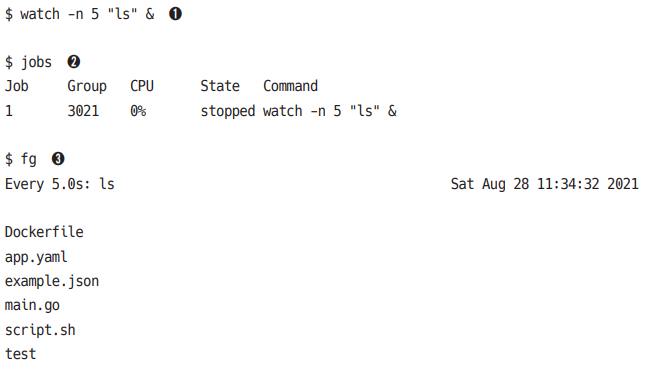
\includegraphics[width=15cm]{resource/3-job-control}
    \label{fig:job-control}
    \begin{enumerate}
        \item 명령 끝에 \&를 넣으면 백그라운드에서 명령이 실행된다.
        \item 모든 작업(job)의 목록을 출력한다.
        \item fg 명령을 사용하면 프로세스를 foreground로 가져올 수 있다.
            watch 명령을 종료하려면 Ctrl+c를 사용한다.
    \end{enumerate}
\end{figure}

\begin{flushleft}
    셸을 닫은 후에도 백그라운드 프로세스를 계속 실행하려면 nohup 명령을 앞에 추가하면 된다.
    또한, 이미 실행 중이지만 앞에 nohup이 붙지 않은 프로세스의 경우에는
    이미 실행 이후라도 \textbf{disown}을 사용하면 동일한 효과를 얻을 수 있다.
    마지막으로 실행 중인 프로세스를 제거하려면 다양한 수준의 강제성과 함께 kill 명령을 사용할 수 있다.
\end{flushleft}

\subsection*{모던 리눅스 명령어}
\begin{flushleft}
    자주 사용되는 명령 중 일부는 대체될 수 있는 모던 명령어가 존재한다.
    drop-in 교체도 존재하고, 일부는 기능을 확장한 것도 존재한다.
    다만, 어떤 도구를 선택할지 고민이 된다면 사용하는 리눅스 배포판에서
    이미 검증된 도구를 사용하는 것이 가장 좋은 방법이다.
\end{flushleft}

\begin{flushleft}
    책과 별개로 개인적인 의견을 남긴다.
    아래 제공되는 모던 리눅스 명령어는 배포판에 default로 설치되는 경우가 아닌경우가 많다.
    따라서 설치 후 사용해야하는 경우가 많고, 이는 일반적인 스크립트 작성에 활용하기 어렵다는 것이다.
    즉, 일반적으로 활용은 어렵다.
\end{flushleft}

\begin{flushleft}
    결론적으로, 실제 활용하기엔 제약이 존재하므로 책의 모든 부분을 작성할 계획은 없으며
    간략한 소개에 그칠 것이다.
\end{flushleft}

\subsubsection*{exa로 디렉터리 내용 나열하기}
\begin{flushleft}
    디렉터리에 무엇이 들어 잇는지 알고 싶으면 ls 혹은 그 변형 중 하나를 매개변수와 함께 사용한다.
    이에 대응하는 모던 리눅스 명령어가 있는데 exa이다.
\end{flushleft}

\subsubsection*{bat로 파일 내용 보기}
\begin{flushleft}
    cat 명령어의 대안으로 bat 명령어 사용을 고려해볼 수 있다.
    bat 명령은 구문을 강조하여 표시할 수 있으며 자체 pager 기능이 존재한다.
\end{flushleft}

\begin{figure}[H]
    \centering
    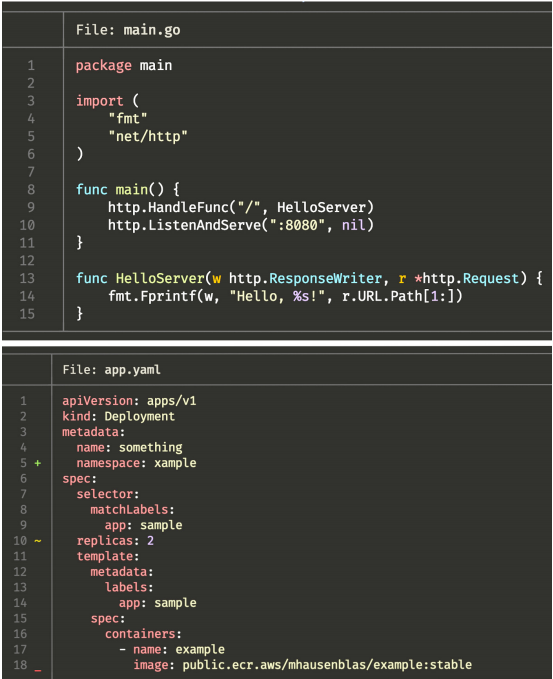
\includegraphics[width=15cm]{resource/3-bat-example.png}
    \caption{bat으로 렌더링한 Go 파일과 YAML 파일}
    \label{fig:bat-example}
\end{figure}


\subsection*{일반 작업}
\subsubsection*{행 탐색과 조작}
\begin{flushleft}
    셸 프롬프트에 명령을 입력할 때는 행을 탐색하거나 행을 조작하는 등 다양한 작업을 한다.
    아래의 표는 일반적으로 사용되는 셸의 단축키 목록이다.
\end{flushleft}


\begin{table}[H]
    \everyrow{\hline}
    \begin{tabu}{|X[7]|X[3]|X[5]|}
        동작 & 명령어 & 비고 \\
        행의 시작으로 커서 이동 & Ctrl+a & - \\
        행의 마지막으로 커서 이동 & Ctrl+e & - \\
        커서를 한 문자 앞으로 이동 & Ctrl+f & - \\
        커서를 한 문자 뒤로 이동 & Ctrl+b & - \\
        커서를 한 단어 앞으로 이동 & Alt+f & 왼쪽 Alt에서만 작동 \\
        커서를 한 단어 뒤로 이동 & Alf+b & - \\
        현재 문자 삭제 & Ctrl+d & - \\
        커서 왼쪽 문자 삭제 & Ctrl+h & - \\
        커서 왼쪽 단어 삭제 & Ctrl+w & - \\
        커서 오른쪽의 모든 항목 삭제 & Ctrl+k & - \\
        커서 왼쪽의 모든 항목 삭제 & Ctrl+u & - \\
        화면 지우기 & Ctrl+l & clear 명령과 동일 \\
        명령어 취소 & Ctrl+r & SIGINT 시그널 전송 \\
        실행 취소 & Ctrl+\_ & bash만 해당 \\
        기록 검색 & Ctrl+r & 일부 셸만 해당 \\
        검색 취소 & Ctrl+g & 기록 검색에 대응함 \\
    \end{tabu}
    \caption{단축키 목록}
    \label{tab:shortcut}
\end{table}

\begin{flushleft}
    모든 단축기가 모든 셸에서 지원되는 것은 아니며 셸마다 다르게 구현될 수 있다.
    이런 단축키는 Emacs 편집 키 입력을 기반으로 한다.
    만약 vi 키 입력을 기반으로 하고 싶다면 .bashrc 파일에 \textbf{set -o vi}를 사용하면 된다.
\end{flushleft}

\subsubsection*{파일 내용 관리}
\begin{flushleft}
    vi 같은 편집기를 사용하지 않고도 텍스트를 편집할 수 있다.
\end{flushleft}

\begin{figure}[H]
    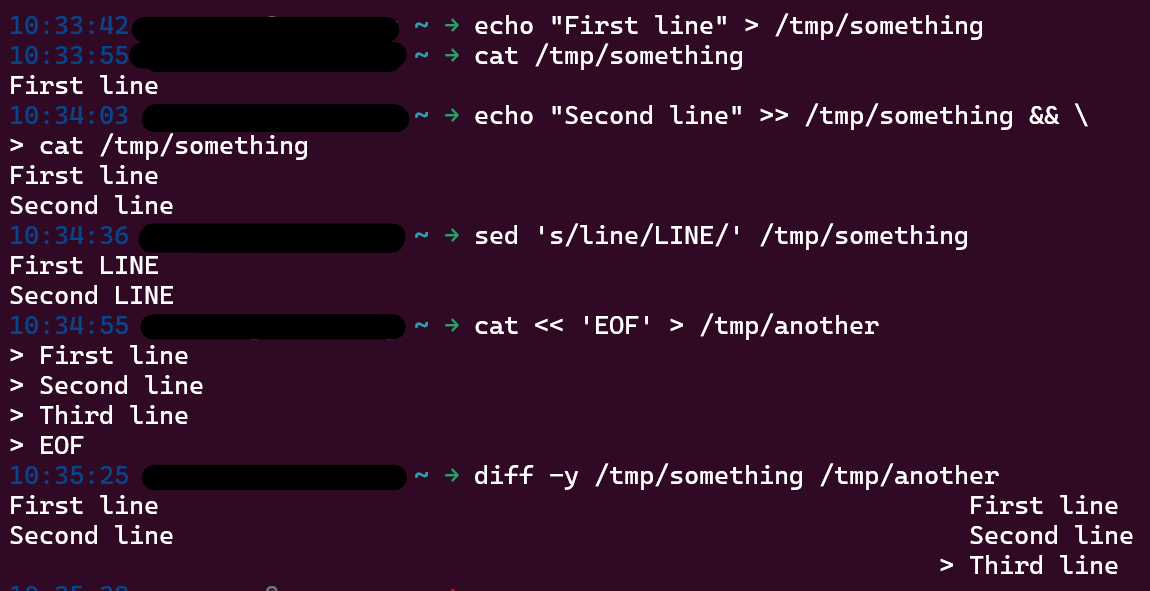
\includegraphics[width=15cm]{resource/3-file-management}
    \label{fig:file-manament}
    \begin{enumerate}
        \item echo 출력을 재지정해 파일을 생성한다.
        \item 파일 내용을 확인한다.
        \item 파일에 한 행을 추가한 후 내용을 확인한다.
        \item sed를 사용해 파일 내용을 바꾸고 stdout으로 출력한다.
        \item redirection을 사용해 파일을 생성한다.
        \item 생성한 파일의 차이점을 보여준다.
    \end{enumerate}
\end{figure}


\subsubsection*{긴 파일 보기}
\begin{flushleft}
    셸의 한 화면에 표시할 수 없을 만큼 행 수가 많은 파일의 경우
    less 또는 bat과 같은 pager를 사용할 수 있다.
    페이지 나누기(paging) 기능을 활용하면 프로그램은 출력을 분할해서
    화면에 나타낼 수 있는 분량에 맞게 페이지를 나눠 표시하고,
    각 페이지를 탐색할 수 있는 명령어(다음 페이지 보기, 이전 페이지 보기 등)를 제공한다.
\end{flushleft}

\begin{flushleft}
    긴파일을 처리하는 또 다른 방법으로 \textbf{head}와 \textbf{tail} 명렁어가 있다.
    예를 들어 파일의 시작 부분을 출력하고 싶다면 다음과 같이 실행한다.
\end{flushleft}

\begin{figure}[H]
    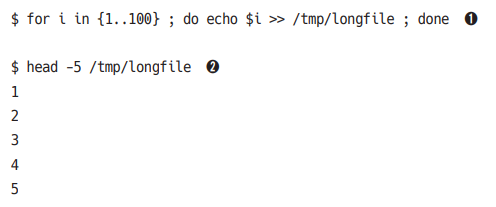
\includegraphics[width=15cm]{resource/3-head-example}
    \label{fig:head-example}
    \begin{enumerate}
        \item 긴 파일을 생성한다(100줄)
        \item 긴 파일의 처음 다섯 행을 출력한다.
    \end{enumerate}
\end{figure}

\begin{flushleft}
    지속적으로 추가되는 파일의 실시간 업데이트를 받으려면 다음을 사용하면 된다.
\end{flushleft}

\begin{figure}[H]
    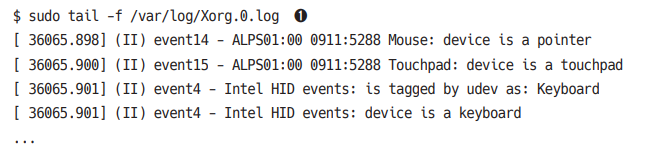
\includegraphics[width=15cm]{resource/3-tail-example}
    \label{fig:tail-exemple}
    \begin{enumerate}
        \item tail을 이용해 로그 파일의 마지막을 출력한다.
            여기서 -f 옵션은 따르다(follow)라는 의미로,
            결과를 지속적으로 확인하거나 자동 업데이트함을 의미한다.
    \end{enumerate}
\end{figure}


\subsubsection*{날짜와 시간 처리}
\begin{flushleft}
    \textbf{date} 명령은 고유한 파일 이름을 생성할 때 유용하다.
    유닉스 타임스탬프 등 여러 형식으로 날짜를 생성하고
    다양한 날짜와 시간 형식 간에 변환할 수도 있다.
\end{flushleft}

\begin{figure}[h]
    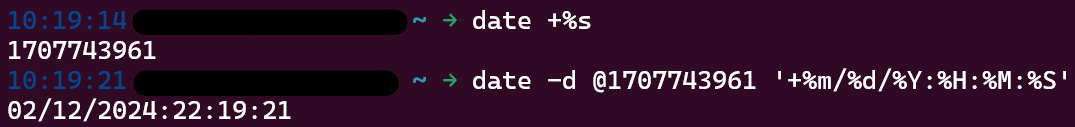
\includegraphics[width=15cm]{resource/3-date-example}
    \label{fig:date-example}
    \begin{enumerate}
        \item 유닉스 타임스탬프를 생성한다.
        \item 유닉스 타입스탬프를 사람이 읽을 수 있는 날짜로 변환한다.
    \end{enumerate}
\end{figure}